\chapter{Introduction}\label{ch:introduction}


Chagas disease is a tropical parasitic epidemic of global reach, spread mostly across 21 Latin American countries. The World Health Organization (WHO) estimates more than six million infected people worldwide~\citep{who2016}. Caused by the \textit{Trypanosoma cruzi} parasite, its transmission occurs mostly in the American endemic regions via the \textit{Triatoma infestans} insect family. It is also known as ``kissing bug'' and ``vinchuca'' in the local variation for Argentina, Bolivia, Chile and Paraguay. In Central America the bug is more commonly known as ``chinche''.
In recent years and due to globalization and migrations, the disease has become an %health
issue in other continents~\citep{schmunis2010chagas},
particularly in countries that receive Latin American immigrants such as Spain~\citep{navarro2012chagas} and the United States~\citep{hotez2013unfolding}.
As a consequence this disease has become a global health problem.


A crucial characteristic of the infection is that it may last 10 to 30 years in an individual without being discovered~\citep{rassi2012american}, which greatly complicates effective detection and treatment.
About 30\% of individuals with chronic Chagas disease will develop any type of symptoms which include life-threatening cardiomyopathies or gastrointestinal disorders.
Long-term human mobility, particularly seasonal and permanent rural-urban migration, play a key role in the epidemic spread~\citep{briceno2009chagas}.
Other relevant routes of transmission include blood transfusion, congenital contagion --with an estimated 14,000 newborns infected each year in the Americas~\citep{OPS2006chagas}--, organ transplants, accidental ingestion of food contaminated by \textit{Trypanosoma cruzi}, and laboratory accidents.

The spatial dissemination of a congenitally transmitted disease sidesteps the available measures to control risk groups, and shows that individuals who have not been exposed to the disease vector should also be included in detection campaigns.
To the best of our knowledge, current studies on human migration patterns in Latin America can provide only coarse and outdated information on user flows at specific municipal levels, without national territory coverage.

In this work, we discuss and explore the use of mobile phone records --also known as Call Detail Records (CDRs)-- for the analysis of mobility patterns and the detection of possible risk zones of Chagas disease in two Latin American countries.
We rely on key health expertise on the subject, provided by the \textit{Mundo Sano} Foundation.
To do this, we will explore the data and rely on a set of different \textit{Machine Learning} tools.
In the remainder of this chapter we will give some key aspects of Chagas disease, and introduce some particular aspects of the countries of our study: Argentina and Mexico.
We will also give a very brief overview of the field of \textit{Machine Learning}.


\section{Mobile Phone Records, Mobility and Epidemiology}

The scientific analysis of mobile phone datasets, collected by operators within their network, is a recent field of study, with a corpus of published works starting in 2005, and a noticeable increase of publications from 2012 onward, as reported in the survey of \citep{naboulsi2015mobile}.
Other milestones of this increased interest of the scientific community are the NetMob conferences, focused on mobile phone data analysis (see \citep{netmob}).

Mobile traffic contains information about the movement, interactions, and mobile service consumption of individuals at unprecedented scales.
This attracted scientists from multiple disciplines:
sociologists, epidemiologists, physicists, transportation and telecommunication experts found in these datasets a clear opportunity to bring their analyses to an unprecedented scale while retaining a high level of detail on each individual.
Thanks to the growing availability of datasets, collaborations between academic research groups and network operators based on the analysis of real-world mobile traffic have been flourishing.
A significant example is the Data for Development Challenges by Orange \citep{d4d} in which CDRs from the telecommunication operator was provided.
This let international research laboratories compete under an innovation challenge whose objective is to contribute to social welfare.

In CDR analysis one of the main research subjects is mobility analysis, where calls can be located by means of knowing cellphone tower geolocalization and by then matching calls to one of these points.
This provides fine granularity projections of users trajectories and in this way users have been found to show a strong regularity in their movement patterns, both in space and time, as described in \citep{gonzalez2008understanding}.

In another study, \citep{song2010limits} explore the limits of predictability in human dynamics by studying the mobility patterns of anonymized mobile phone users.
By measuring the entropy of individuals trajectories, the authors found a 93\% potential predictability in user mobility across the whole user base.

Human mobility is also influenced by social components: \citep{cho2011friendship} observe that social relationships
can explain about 10\% to 30\% of all human movement, while periodic
behavior explains 50\% to 70\%; whereas \citep{ponieman2016mobility} show how social ties can be used to improve mobility predictions, for the case of people attendance to large social events.

Mobility analysis has applications in diverse areas such as urban planning (see \citep{wang2012understanding}) and disaster recovery (see \citep{lu2012predictability}).
In particular, mobile phone records contain information about the movements of large subsets of the population of a country, and make them very useful to understand the spreading dynamics of infectious diseases, while preserving the privacy of users.

For instance, CDRs have been used to understand the diffusion of malaria in Kenya by \citep{wesolowski2012quantifying} and in Ivory Coast by \citep{enns2013human}, including the refining of infection models performed by \citep{chunara2013large}.
The cited works on Ivory Coast were presented using the ``Data for Development'' (\citep{d4d}) challenge datasets released in 2013. \citep{tizzoni2014use} compare different mobility models using theoretical approaches, available census data and algorithms based on CDRs interactions to infer people movements.
They found that the models based on CDRs and mobility census data are highly correlated, illustrating CDR use as mobility proxies.

Mobile phone data has also been used to predict the geographic spread and timing of Dengue epidemics by \citep{wesolowski2015impact}.
This analysis was performed for the country of Pakistan, which is representative of many countries on the verge of countrywide endemic dengue transmission.
Other works directly study CDRs to characterize human mobility and other sociodemographic information.
A complete survey of mobile traffic analysis articles may be found in \citep{naboulsi2015mobile}, which also reviews additional studies based on the Ivory Coast dataset mentioned above.

In this work we intend to show how these data can help in the problem of Chagas disease, by means of accurately describing people migrations and movements at a national level.
We expect to add more relevant information to the problem of detecting \textit{foci} of communities with high rates of prevalence, out of the endemic region.

It is relevant to the purpose of this work to note that specifically tagging disease-carriers is out of scope.
We have no reason to believe that this dataset can provide such information with accuracy and we have not found any data sources to cover this missing  information.

\section{Machine Learning}

Machine learning is a sub-field of computer science with broad \textit{theoretical} intersections with statistics and mathematical optimization.
At present time, it has a wide range of applications.
A non-comprehensive list of its uses includes self-driving cars, Spam detection systems, face and voice recognition, temperature prediction in weather, AI opponents in games, disease detection in patients, text and audio language translation, stock pricing, movie recommendation systems, etc.
Examples of these Machine Learning programs are now widespread to the point where their use today has a direct impact on the daily lives of millions of people.
Due to this, Machine Learning has \textit{practical} intersections with data and software engineering.


\citep{Mitchell-MLearning} gives the following definition of Machine Learning:
``A computer program is said to learn from experience E with respect to some class of tasks T and performance measure P if its performance at tasks in T, as measured by P, improves with experience E''.

For our purposes it is clear though that this definition\footnote{Other authors might reference to Machine Learning as \textit{statistical learning}. See~\citep{hastie-elemstatslearn} as an example.} is not a mathematical one.
However it serves to convey the idea of algorithms that automatically \textit{learn} to do a specific task better over time and with more data.
Note that the ``goodness'' of their performance is inherently subjected to the evaluation criteria chosen for the task.
Because of this, the concept of \textit{learning} within this context is less associated with the cognitive definition and more related to an optimization based approach.

In this thesis we break down our purpose of work into different tasks to generate predictions of population movements between regions.
We give a broad presentation of tools that are necessary to carry out this task and, additionally, we give an introduction to the field's vocabulary, theory and practical notes on how it can be used for this kind of problems.

We later start solving the tasks as we introduce a set of supervised classification algorithms.
All along this work, the idea will be to exemplify the concepts as much as we can with actual work on the CDR data.
Also, we will try to assess what are the best attributes that can be extracted from the data for the prediction tasks.

The problem of long-term human migrations will provide a proxy to understand the spread of Chagas disease.
This work's objective is to show that geolocalized call records are rich in social and individual information, which can in turn be used to determine whether an individual has lived in an epidemic area.
We present two case studies, in Argentina and in Mexico, using data provided by mobile phone companies from each country. %A discussion of how mobile data was processed is included.
To the best of our knowledge, this is the first work that leverages mobile phone data to better understand the diffusion of the Chagas disease.


\section{Key Facts on Chagas Disease}

\subsection{Chagas Disease in  Argentina}\label{endemic_zone_argentina}

For more than 50 years, vector control campaigns have been underway in Argentina as the main epidemic counter-measure.
The \textit{Gran Chaco}, situated in the northern part of the country is home to the disease-carrying triatomines.
This region is hyper-endemic for the disease~\citep{OPS2014mapa}.
A map of this ecoregion is shown in \cref{fig:granchaco}.

\begin{figure}[ht]
\centering
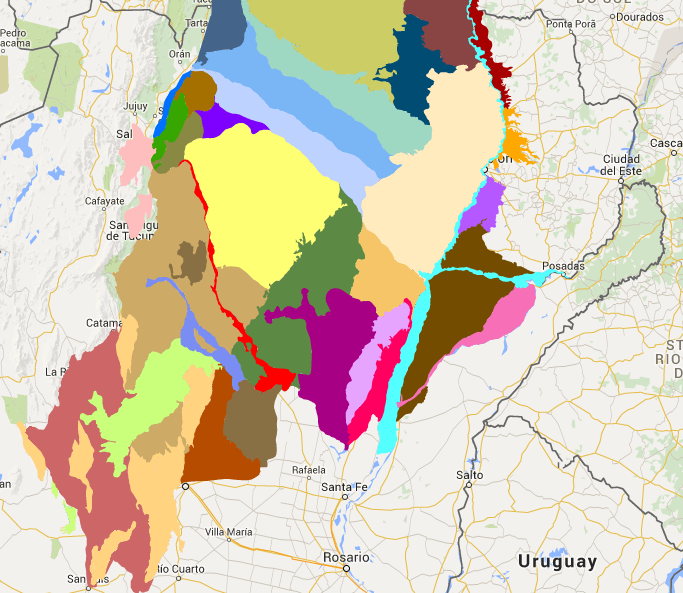
\includegraphics[width=0.75\columnwidth]{figures/Ambientes_GranChaco_TNC-Argentina/Ambientes_GranChaco_TNC-Argentina}
\caption{The \textit{Gran Chaco} ecoregion in South America.%
}
% \end{center}
\label{fig:granchaco}
\end{figure}

The ecoregion's low socio-demographic conditions further support the parasite's life-cycle, where domestic interactions between humans, triatomines and animals foster the appearance of new infection cases, particularly among rural and poor areas.
% The ecoregion as of today is hyper-endemic for the disease.
This region is considered as the endemic zone $E_Z$ in the analysis described in \cref{ch:descr-risk} and \cref{ch:machineLearning}.


The dynamic interaction of the triatomine infested areas and the human mobility patterns create a difficult scenario to track down individuals or spots with high prevalence of infected people or transmission risk.
Available methods of surveying the Chagas disease state in Argentina are nowadays limited to screenings of individuals.

Recent national estimates indicate that there exist between 1.5 and 2 million people carrying the parasite, with more than seven million exposed. National health systems face many difficulties to effectively treat the disease.
In Argentina, less than 1\% of infected people are diagnosed and treated
(the same statistic holds at the world level).

Even though governmental programs have been ongoing for years now~\citep{plan_nacional_chagas}, data on the issue is scarce or of difficult access.
This presents a real obstacle to ongoing research and coordination efforts to tackle the disease in the region.


\subsection{Chagas Disease in  Mexico}\label{endemic_zone_mexico}


In 2004, the joint work of \textit{Instituto Nacional de Cardiología ``Ignacio Chávez''} and  \textit{Instituto de Biología de la UNAM} resulted in a Chagas disease database for Mexico (\citep{cruz2006chagmex}).
Reviewing positive serology in blood banks and human reported cases per state, an epidemic risk map description was produced to geographically situate the disease.
Based on this data, we defined the Mexican epidemic area, selecting the states having the top 25\% prevalence rates nationwide.
The resulting risk region is shown in \cref{fig:endemic_zone_mexico}.
It covers most of the Southern region of the country and includes the states of Jalisco, Oaxaca, Veracruz, Guerrero, Morelos, Puebla, Hidalgo and Tabasco.
This region is considered as the endemic zone $E_Z$ for the Mexican case in the analysis described in~\cref{ch:descr-risk} and \cref{ch:machineLearning}.

\begin{figure}[ht]
\centering
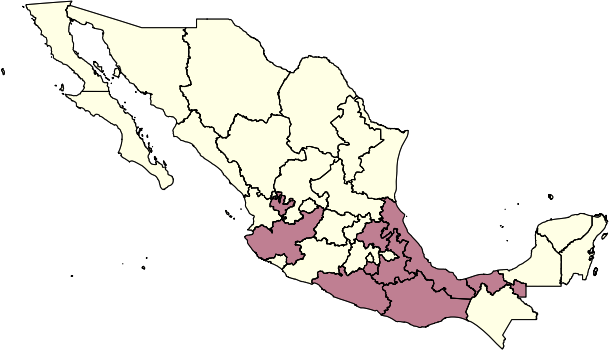
\includegraphics[width=0.75\linewidth]
{figures/Ambientes_Gran_Chaco-Mexico1/Ambientes_Gran_Chaco-Mexico1}
\caption{Endemic region $E_Z$ for Mexico.}
\label{fig:endemic_zone_mexico}
\end{figure}


The authors of~\citep{carabarin2013chagas} provide an extensive review of the
research reports on Chagas disease in Mexico.
The review is very critical, stating that there are no effective vector control programs in Mexico; and that the actual prevalence of the disease
can only be estimated because no official reporting of cases is performed.

According to~\citep{dumonteil1999update}, there are a total of 18 endemic areas in Mexico, located in the southeast, and these areas include the states of Oaxaca, Jalisco, Yucatán, Chiapas, Veracruz, Puebla, Guerrero, Hidalgo, and Morelos, all of them with rural areas.
Chiapas, Oaxaca, Puebla, Veracruz and Yucatán are among the most affected states (where the prevalence may exceed 10\%), although cases have been reported in most areas of the country (\citep{cruz2006chagmex,dumonteil1999update}).
Despite the lack of official reports, an estimate for the number of \textit{Trypanosoma cruzi} infections by state in the country
indicates that the number of potentially
affected people in Mexico is roughly 5.5 million (see~\citep{carabarin2013chagas}).
Mexico, together with Bolivia, Colombia, and Central
America, are among the countries most affected by this
\textit{neglected tropical disease} (NTD), as reported by~\citep{hotez2013innovation}.
For what we know, nowadays the disease spreads across borders:
Chagas and other neglected tropical diseases present in the north of Mexico remain highly endemic in the south of Texas as well (\citep{hotez2012texas}).

In recent years there has been a focus on treating the disease with two available medications, benznidazole or nifurtimox.
A study that explores the access to these two drugs in Mexico
shows that less than 0.5\% of those who are infected with
the disease received treatment in Mexico in years (\citep{manne2013barriers}).


People from endemic areas of Chagas disease tend to migrate to industrialized cities of the country, mainly Mexico City, in search of jobs.
In accordance with this movement, \citep{guzman2001epidemiology} showed
that infected children under 5 year of age are frequently distributed in urban
rather than in rural areas, indicating that the disease is becoming urbanized in
Mexico.
Therefore, as in the Argentinian case, the study of long-term mobility is crucial to understand the spread of Chagas disease in Mexico.



\section{Thesis Structure}


\cref{ch:descr-risk} will present the data sources and give the main idea behind how we process the data.
It will also show some basic descriptive aspects of the information that can be found in the CDR logs and how it compares to other data sources.
Finally, the chapter will develop the methodology used to construct chagasic national disease risk maps from the data logs.
Examples of maps will be shown to illustrate the results found.

In \cref{ch:machineLearning} we will give a more in-depth introduction to Machine Learning theory, describing use cases, ideas and concepts from this field.
Our long-term migration prediction tasks will be formulated in a way that can be used in a binary classification problem that can be later input to a statistical model.
Added to this, we will introduce Machine Learning theory along with examples of applications on the processed dataset.
We will use various examples with the Logistic Regression classifier in order to illustrate the concepts involved.

\cref{ch:modelSelection} will further expand concepts from the field of Machine Learning that will be used throughout our analyses.
We will also give an overview of different strategies to select the best statistical models.
% and we will make a very brief mention on Vapnik-Chervonenkis'  Statistical Learning Theory, to set.

\cref{ch:ensembleMethods} will concentrate on specific tree-based algorithms for Supervised Machine Learning Classification tasks.
We will introduce the minimal formulations for the models, as well as their applications.
For each of these, we will dive into their main benefits and drawbacks, and we will compare all of them under a common classification problem.
Finally, along with the presentation of each method, we will show specific long-term human migration experiments on the CDR data,
For each case we will show the results of these applications and the discoveries made.
Additionally, we will introduce the Naive Bayes as a model on which to benchmark.

We close this work with a summary of results in \cref{ch:results} where key information from the previous chapters' output is recollected.
We then give this work's conclusions in \cref{ch:conclusions}, along with drawbacks from the methodology used and possible lines of future work.



